\section{Grafos Expansores}
\begin{frame}
  \begin{itemize}[<+-| alert@+>] 
    \item Existem muitas definições de grafos expansores
    \item Todas tem uma mesma ideia: grafo esparso e altamente conexo 
    \item Vamos ver uma das possíveis definições 
  \end{itemize}
\end{frame}

\subsection{Expansão}

\begin{frame}{Altamente conectado}
  Precisamos definir a ideia de um grafo altamente conexo:
  \onslide<2->{%
    \begin{center}
    \huge Que tal o número o número de corte??
    \end{center}
  }
\end{frame}

\begin{frame}
  \begin{example}
    Considere o seguinte grafo $(n \ge 100)$:
    \begin{center}
      \begin{tikzpicture}
        \node[draw, ellipse, minimum width=2cm, minimum height=5cm, label=center:$K_n$] (A) at (0,0) {};
        \node[draw, ellipse, minimum width=2cm, minimum height=5cm, label=center:$K_n$] (B) at (6,0) {};
        \draw (A.east) -- (B.west);
        \node at (3,0.8) {100 arestas};
        \visible<2->{%
          \node[anchor=west] at (8,0) {$\lim_{n\rightarrow +\infty}{\frac{\lambda(K_n)}{|K_n|}} = 0$};
        }
    \end{tikzpicture}
  \end{center}
\end{example}
\end{frame}

\begin{frame}{Constante de Cheeger ou Razão de Expansão}
  Precisamos de outra forma de medir isso:  
  \visible<2->{%
    \begin{definition}[Constante de Cheeger]
      Seja $G = (V, E)$ um grafo. A constante de Cheeger de $G$, denotada por $h(G)$, é definida por
      \[
        h(G) = \min_{S\subsetneq V }\frac{|\partial S|}{\min(|S|, |V|\setminus|S|)}
      \]
    \end{definition}
  }
\end{frame}

\begin{frame}
  \begin{example}
    Considere o grafo completo $K_n$ e $S \subset V$ um subconjunto com m
    vertíces, temos que:

    \[
      |\partial S| = m(n-m)
    \]

    Então:

    \[
      \frac{|\partial S|}{\min(|S|,|V|\setminus|S|)} =\frac{m(n-m)}{\min(m, n-m)} = \max(m , n - m).
    \]

    O valor que minimiza a expressão é $m=\frac{n}2$, logo teremos que:

    \[
        h(K_n) = \frac{n}2
    \]

    \vspace{5pt}

  \end{example}
\end{frame}

\begin{frame}{Grafo $c-expansor$}
  \begin{definition}[Grafo $c-expansor$]
    Seja $G$ um grafo $c > 0$ uma constante, G é um grafo $c-expansor$ se $h(G)
    \ge c$
  \end{definition}

  \vspace {10pt}
  \visible<2->{
  Poderiamos aqui definir uma classe de grafos, os grafos que são
  $c-expansores$, o objeto que é verdeidaramente interessante reside nessas classes
}
\end{frame}

\begin{frame}{Hmmm...}
  \begin{itemize}[<+-| alert@+>] 
    \item Todo grafo $G$ é um grafo $h(g)-expansor$ (se $G$ é conexo)
    \item Estamos interessados nos grafos com $h(G)$ grande?
    \item Lembre do $K_n$: $h(G)$ grande mas com muitas arestas
    \item Onde entra a esparsidade? 
  \end{itemize}

  \vspace{10pt}
  \visible<5->{%
    \begin{center}
    \Large Na verdade, o que importa é a familia... \\
    \vspace{10pt}
    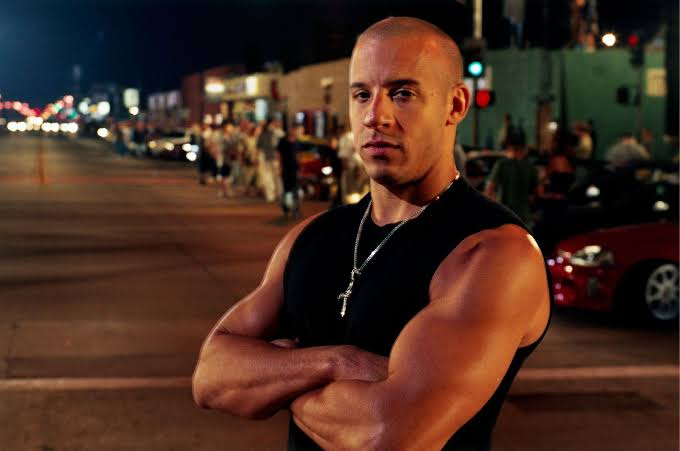
\includegraphics[width=0.3\linewidth]{pic/vin_diesel.jpeg}
    \end{center}
  }
\end{frame}

\begin{frame}
  \begin{definition}[Família de grafos expansores]
Uma família de grafos finitos $d$-regulares\footnote{Poderia se usar uma definição mais forte que só limita o grau dos vértices} $\{G_i\}_{i\in\mathbb{N}}$ com $\lim_{i\to\infty} |G_i| = \infty$ é uma família de grafos expansores se existe $c >0$ tal que, para todo $i\in\mathbb{N}$, $G_i$ é $c$-expansor.
\end{definition}

\end{frame}

\begin{frame}{Agora sim...}

  \begin{itemize}[<+-| alert@+>] 
    \item Número de arestas é linear no número de vértices 
    \item Garante um nível de conexidade independente do tamanho do grafo
  \end{itemize}
\end{frame}

\subsection{Expansão e a lacuna espectral}

\begin{frame}{Inequação de Cheeger}
\begin{theorem}[Inequação de Cheeger]
\label{thm:cheeger}
Seja $G$ um grafo $d$-regular e $\lambda_1\ge \lambda_2 \ge \dots \ge \lambda_n$ seu espectro. Então
\[
\frac{d-\lambda_2}{2}\leq h(G) \leq \sqrt{2d(d-\lambda_2)}.
\]
\footnotetext{Lembre que $d-\lambda_2 $ é a lacuna espectral}
\end{theorem}
\vspace{10pt}
\visible<2->{
  \begin{center}
  \large A constante de cheeger está intimamente relacionada a lacuna espectral
  \end{center}
}
\end{frame}

\section{Grafos expansores e o tempo de mistura}

\subsection{Expansão e o tempo de mistura}

\begin{frame}
  Seja $G=(V,E)$ um grafo $d$-regular conexo e $\lambda_1\ge \lambda_2 \ge \dots
  \ge \lambda_n$ seu espectro, considere um passeio aleatório
  preguiçoso em G com matriz de transição P, lembre que lacuna espectral de P é a seguinte:

\[
\gamma = \frac{d-\lambda_2}{2d}
\]

\visible<2->{
Então substituindo na inequação de Cheeger:
\[
d\gamma  \leq h(G) \leq \sqrt{(2d)^2\gamma} \implies 
d\gamma  \leq h(G) \leq 2d\sqrt{\gamma}
\]
}

\visible<3->{
Logo a constante de Cheeger está relacionada a lacuna espectral do passeio
}
\end{frame}

\begin{frame}{Relemebrando...}
  \begin{center}
  A lacuna espectral do passeio determina o tempo de mistura:
\[
  \mathcal{O}\!\left(\frac{1}{\gamma}\log n\right).
\]

Portanto a constante indiretamente irá defninir o tempo de mistura.

\vspace{20pt}
\visible<2->{
\large \textcolor{red}{A constante de cheeger é inversamente
proporcional ao tempo de mistura}
}
  \end{center}
\end{frame}

\subsection{Famílias e o tempo de mistura}
\begin{frame}
\begin{theorem}
Seja $\{G_i=(V_i, E_i)\}_{i\in\mathbb{N}}$ uma família de grafos $c-expansores$
$d$-regulares. Então um passeio aleatório preguiçoso $P$ em $G_i$ possui tempo de
mistura $ O(\log |V_i|)$.
\end{theorem}
\end{frame}

\begin{frame}
  \begin{proof}
    Seja $\gamma_i$ a lacuna espectral de $P$, podemos derivar da inequação
    anterior:
    \visible<2->{
      \[ 
        d\gamma_i  \leq h(G_i) \leq \sqrt{(2d)^2\gamma_i} \implies 
      \frac{h(G_i)^2}{4d^2} \leq \gamma_i\]
    }
    \visible<3->{%
      Por definição de família expansora, existe $c>0$ tal que $h(G_i)\geq c$ para todo $i$. Então:

      \[ \frac{c^2}{4d^2} \leq\frac{h(G_i)^2}{4d^2} \leq \gamma_i \implies
      \frac{4d^2}{c^2}  \ge \frac1\gamma_i\]
    }
    \visible<4->{%
      A cota geral para o tempo de mistura discutida anteriormente nos dá
      \[
        \tau_{\mathrm{mix}}(\varepsilon) =  \mathcal{O}\!\left(\frac{1}{\gamma_i}\log |V(G_i)|\right) 
        \implies \tau_{\mathrm{mix}}(\varepsilon) = O(\log |V(G_i)|)
      \]
      Como $1/\gamma_i$ é limitado por uma constante, é absorvido pela notação assintótica.    
    }
  \end{proof}
\end{frame}

\section{Conclusão}

\begin{frame}
  Vimos:
  \begin{itemize}[<+-| alert@+>] 
    \item O que é o tempo de mistura de um passeio 
    \item O que é uma família de grafos expansores
    \item Como esses dois conceitos se relacionam por meio dos seus espectros 
  \end{itemize}
  \vspace{10pt}
  \visible<4->{
    Concluimos então:
  \begin{center}
    \large\textcolor{red}{As famílias de grafos expansores são uma ferramenta
    para adquirir grafos arbitrariamente grandes com poucas arestas e com tempo
  de mistura pequeno.}
  \end{center}
}
\end{frame}

